\RequirePackage{fix-cm}
\documentclass[smallextended]{svjour3}
\smartqed
\usepackage{amsmath,amssymb,graphicx,booktabs,array,longtable}
\usepackage[numbers,sort&compress]{natbib}
\usepackage{url}
\usepackage{float}
\floatstyle{ruled}
\newfloat{algorithm}{tbp}{loa}
\floatname{algorithm}{Algorithm}
\usepackage[hidelinks]{hyperref}
\journalname{Autonomous Agents and Multi-Agent Systems}
\usepackage{xr}
\externaldocument[main-]{../main}
\newcommand{\E}{\mathbb{E}}
\newcommand{\U}{U}
\newcommand{\ind}{\mathbf{1}}
\newcommand{\authorinput}[1]{\textbf{AUTHOR INPUT NEEDED: #1}}
\setlength{\emergencystretch}{3em}
\raggedbottom
\clubpenalty=10000
\widowpenalty=10000
\hypersetup{pdftitle={Online Resource 1: Supplementary Material for Auditing the Value of Delayed Advice in Autonomous Agents},pdfsubject={Delayed Advice Audit},pdfkeywords={Delayed Advice Audit, supplementary material}}

\renewcommand{\thetable}{S\arabic{table}}
\renewcommand{\thefigure}{S\arabic{figure}}
\begin{document}
\title{Online Resource 1: Supplementary Material for Auditing the Value of Delayed Advice in Autonomous Agents}
\titlerunning{Delayed Advice Audit: Supplementary Material}
\author{Author information pending}
\institute{Companion to the delayed-advice audit article.}
\date{}\maketitle
This resource preserves detailed experimental methods, every reported condition, numerical selection grids, historical source-budget studies and engineering provenance. It supports the compact main article without supplying additional independent cohorts. Section and table references without an S prefix refer to the main article. Current visual-channel and temporal extensions are documented after the retained evidence; historical protocols remain distinguishable.
\section{Technical conventions beyond the main article}
The original visual source and all four local heads use the same whole-episode demonstration partition. Local action heads and pose heads differ in target supervision; pose estimates become actions through the public task controller. The fixed deployed local action-head capacities are 16/128 on Push and 32/256 on PickPlace. Full architecture and optimization details are retained below.

Visual arrival inputs use request and arrival $512\times16\times16$ feature maps, robot states and their difference, all four head predictions at both times, and three clock terms. Packet enrichment adds 400 coordinates. A single named source option can execute a different action sequence when its packet changes, even with an invariant gate. State critics instead receive 58 local features or 62 with the four-dimensional packet. Snapshot reward bookkeeping and native success are never online critic inputs.

State sensor noise affects hand/object/goal positions independently at each native step; gripper opening is unnoised. Paired branches use the same time-indexed Gaussian stream. This is coordinate noise, not semantic feedback corruption. Repeated requests at 16/144/272/400 have spacing 128, exceeding the maximum delay-plus-hold $64+32$. Later public-source packets can diverge with closed-loop states across policies; periodic evaluation therefore does not assume identical future messages.

Native state branches use prefix reuse only for exactly identical actions and future noise. Six boundary smoke cases independently execute all 22 learned/reference policies sequentially and compare complete reward/action traces with the reused tree. These cases are excluded from scientific samples. State NumPy critic exports agree with Torch to $1.78\times10^{-15}$ on the checked training/validation inputs.

The larger-budget visual replication trains all 15,000 updates before validation-only source selection. It restarts optimization from the common pretrained initialization rather than resuming archived 3k weights without optimizer state. First-3k loss histories match their earlier counterparts excluding elapsed time. New actor seeds generate their own arrival labels on the same development environment/clock pool. All 160 model/config files are frozen before testing, including engineering tests. No weaker source or trained system is discarded.

The original and current code fingerprints, version changes and failed fit/recovery records remain separated in the archive. Engineering replay validates the executed local configuration; it does not establish simulator correctness or clean-machine portability. The source-data manifest links every quantitative table to its analyzed records.

\section{Additional results and inference details}\label{s-app:inference}
\subsection{Original exact event bounds}
For each paired reward difference $D$, define $p=\Pr(D>10^{-10})$. With rewards in 0--10, $D\leq10$ implies $\E[D]\leq10^{-10}+10p$. A one-sided Clopper--Pearson upper bound $p_U$ therefore yields the conservative mean-positive-part bound $10^{-10}+10p_U$. Six such bounds received error $0.05/12$ each, complementing the six approximate bootstrap intervals with the same allocation. All six bounds were too loose to exclude the prespecified 0.25 reward-scale gain. The union-bound allocation for exact event bounds does not make the percentile-bootstrap intervals distribution-free. Sparse nonzero differences, notably 10 and 16 cases for the first two Push contrasts, further limit their interpretation. No finite-sample safety, equivalence or universal non-benefit result is claimed.

\subsection{Supplementary curves, contrasts and figures}
\begin{figure}[H]
\centering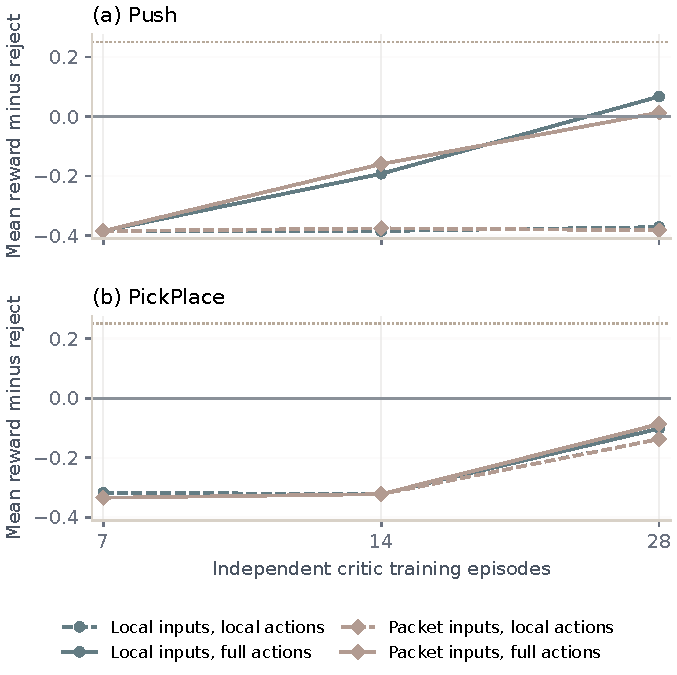
\includegraphics[width=\textwidth]{../figures/critic_learning_curve.pdf}
\caption{Descriptive critic-data learning curves, using a common fresh test pool within each task. Training sets are nested, with the same 12 validation episodes. The actor remains training seed 0. The dotted 0.25 line is an investigator-defined reward-scale reference, not a validated operational utility threshold. Primary uncertainty is reported in Table~\ref{s-tab:curveall}.}\label{s-fig:curve}
\end{figure}



Table~\ref{s-tab:curveall} retains the complete eight-contrast family. All models were fitted and frozen before the independent test environments. Zero model selection in the original 14/6 cohort does not imply zero selection in this 28/12 cohort. A sample-size comparison within this new nested draw is different from comparing the old and new development cohorts.
\begin{table}[H]\centering\small
\caption{All learning-curve primary contrasts, approximate 99.375\% intervals.}\label{s-tab:curveall}
\begin{tabular}{llrr}
\toprule Task & Contrast & Mean & Interval\\\midrule
Push & 28full--reject & +0.013 & [-0.566,+0.593]\\
Push & 28full--14full & +0.173 & [-0.494,+0.862]\\
Push & 28packet/local input & -0.011 & [-0.057,+0.000]\\
Push & 28full/local action & +0.396 & [-0.173,+0.968]\\
PickPlace & 28full--reject & -0.087 & [-0.333,+0.155]\\
PickPlace & 28full--14full & +0.235 & [-0.063,+0.568]\\
PickPlace & 28packet/local input & -0.000 & [-0.121,+0.128]\\
PickPlace & 28full/local action & +0.050 & [-0.130,+0.238]\\
\bottomrule\end{tabular}\end{table}


\begin{figure}[H]
\centering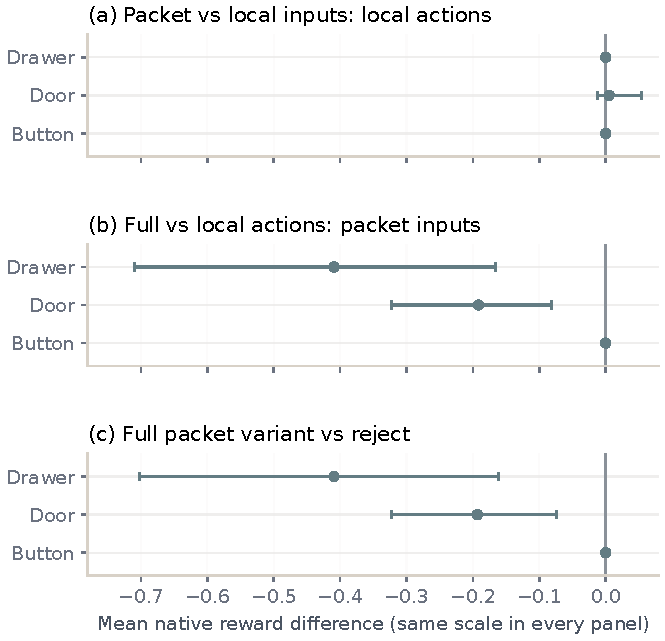
\includegraphics[width=\textwidth]{../figures/state_contrasts.pdf}
\caption{State-cohort policy contrasts averaged over five critic initializations and the 12 equally weighted delay/frequency/noise conditions. Points and intervals report the predeclared approximate stratified crossed-bootstrap analysis. Zero-width results on Button and the Drawer input contrast have structural null-policy explanations; a degenerate bootstrap is not itself an equivalence proof. All panels use the same horizontal reward-difference scale. Raw reward differences are kept separate by task.}\label{s-fig:state}
\end{figure}

\subsection{State-cohort condition breakdowns}
Tables~\ref{s-tab:drawerbreak}--\ref{s-tab:buttonbreak} retain every predeclared condition. These are descriptive averages over five critic seeds and ten environments/cell. Each cell has fresh environment seeds; policy comparisons are paired within a cell, while the delay/frequency/noise entries are not a same-environment factorial crossover. Subgroup point differences are not promoted to new primary tests or used to revise models. All full-state-cohort means, seed-level contrasts, success counts and packet-probe counts are in the accompanying JSON source data.
\begin{table}[H]\centering\small
\caption{Drawer descriptive condition means. $I=P,C-L,C$, $A=P,F-P,C$, $T=P,F-R$. $d$:native steps,noise:metres.}\label{s-tab:drawerbreak}
\begin{tabular}{rllrrr}
\toprule $d$ & Schedule & Noise & $I$ & $A$ & $T$\\\midrule
0 & single & 0.000 & +0.000 & -0.002 & -0.002\\
0 & single & 0.005 & +0.000 & -0.002 & -0.002\\
0 & periodic & 0.000 & +0.000 & -0.016 & -0.016\\
0 & periodic & 0.005 & +0.000 & -0.255 & -0.255\\
16 & single & 0.000 & +0.000 & -0.011 & -0.011\\
16 & single & 0.005 & +0.000 & -0.039 & -0.039\\
16 & periodic & 0.000 & +0.000 & -0.114 & -0.114\\
16 & periodic & 0.005 & +0.000 & -0.290 & -0.290\\
64 & single & 0.000 & +0.000 & -1.174 & -1.174\\
64 & single & 0.005 & +0.000 & -1.019 & -1.019\\
64 & periodic & 0.000 & +0.000 & -0.782 & -0.782\\
64 & periodic & 0.005 & +0.000 & -1.207 & -1.207\\
\bottomrule\end{tabular}\end{table}
\begin{table}[H]\centering\small
\caption{Door descriptive condition means. $I=P,C-L,C$, $A=P,F-P,C$, $T=P,F-R$. $d$:native steps,noise:metres.}\label{s-tab:doorbreak}
\begin{tabular}{rllrrr}
\toprule $d$ & Schedule & Noise & $I$ & $A$ & $T$\\\midrule
0 & single & 0.000 & -0.004 & +0.002 & -0.004\\
0 & single & 0.005 & -0.005 & +0.006 & +0.005\\
0 & periodic & 0.000 & +0.064 & -0.167 & -0.168\\
0 & periodic & 0.005 & +0.001 & -0.887 & -0.896\\
16 & single & 0.000 & +0.004 & -0.002 & -0.002\\
16 & single & 0.005 & -0.001 & -0.002 & +0.002\\
16 & periodic & 0.000 & -0.025 & -0.025 & -0.019\\
16 & periodic & 0.005 & +0.031 & -0.190 & -0.188\\
64 & single & 0.000 & +0.002 & -0.035 & -0.035\\
64 & single & 0.005 & -0.005 & -0.028 & -0.037\\
64 & periodic & 0.000 & -0.003 & -0.347 & -0.351\\
64 & periodic & 0.005 & +0.003 & -0.624 & -0.627\\
\bottomrule\end{tabular}\end{table}

\begin{table}[H]\centering\small
\caption{Button descriptive condition means. $I=P,C-L,C$, $A=P,F-P,C$, $T=P,F-R$. $d$:native steps,noise:metres.}\label{s-tab:buttonbreak}
\begin{tabular}{rllrrr}
\toprule $d$ & Schedule & Noise & $I$ & $A$ & $T$\\\midrule
0 & single & 0.000 & +0.000 & +0.000 & +0.000\\
0 & single & 0.005 & +0.000 & +0.000 & +0.000\\
0 & periodic & 0.000 & +0.000 & +0.000 & +0.000\\
0 & periodic & 0.005 & +0.000 & +0.000 & +0.000\\
16 & single & 0.000 & +0.000 & +0.000 & +0.000\\
16 & single & 0.005 & +0.000 & +0.000 & +0.000\\
16 & periodic & 0.000 & +0.000 & +0.000 & +0.000\\
16 & periodic & 0.005 & +0.000 & +0.000 & +0.000\\
64 & single & 0.000 & +0.000 & +0.000 & +0.000\\
64 & single & 0.005 & +0.000 & +0.000 & +0.000\\
64 & periodic & 0.000 & +0.000 & +0.000 & +0.000\\
64 & periodic & 0.005 & +0.000 & +0.000 & +0.000\\
\bottomrule\end{tabular}\end{table}


\subsection{Development tolerance and descriptive delay strata}
\begin{table}[H]\centering\small
\caption{Zero-predictor selections among 100 preassigned 14/6 resplits of the original 20 development environments per task. Columns vary model-selection MSE tie tolerance, not the deployment acceptance threshold. These reuse development outcomes and are not independent test-performance estimates.}\label{s-tab:tolerance}
\begin{tabular}{llrrrrr}\toprule Task & Cell & $0$ & $10^{-14}$ & $10^{-12}$ & $10^{-10}$ & $10^{-8}$\\\midrule
Push & $L,C$ & 3 & 3 & 3 & 3 & 5\\
Push & $L,F$ & 2 & 3 & 4 & 4 & 6\\
Push & $P,C$ & 2 & 2 & 2 & 2 & 4\\
Push & $P,F$ & 2 & 2 & 2 & 3 & 5\\
PickPlace & $L,C$ & 5 & 7 & 11 & 13 & 15\\
PickPlace & $L,F$ & 4 & 5 & 7 & 9 & 10\\
PickPlace & $P,C$ & 13 & 14 & 17 & 19 & 19\\
PickPlace & $P,F$ & 6 & 6 & 9 & 10 & 10\\
\bottomrule\end{tabular}\end{table}

\begin{table}[H]\centering\small
\caption{Archived original validation grid diagnosis. Each cell compares the zero predictor with the strict best of 12 nonzero bandwidth/ridge candidates. $\delta=\mathrm{MSE}_0-\min\mathrm{MSE}_{\mathrm{nonzero}}$; positive $\delta$ means zero is worse. MSE targets are native gains divided by ten. Final selection uses the global $10^{-12}$ tie pool, so it may differ from the strict minimum. No alternative policy was tested here.}\label{s-tab:hypergrid}
\begin{tabular}{llrrrl}\toprule Task & Cell & Best $h$ & Best $\lambda$ & $\delta$ & Selected\\\midrule
Push & $L,C$ & 4 & 1 & +5.03e-03 & RBF\\
Push & $L,F$ & 4 & 1 & +3.33e-03 & RBF\\
Push & $P,C$ & 4 & 1 & +5.07e-03 & RBF\\
Push & $P,F$ & 4 & 1 & +3.39e-03 & RBF\\
PickPlace & $L,C$ & 1 & 10 & +1.61e-05 & RBF\\
PickPlace & $L,F$ & 1 & 1 & +1.03e-03 & RBF\\
PickPlace & $P,C$ & 0.25 & 0.01 & +1.43e-13 & zero\\
PickPlace & $P,F$ & 1 & 1 & +1.77e-04 & RBF\\
\bottomrule\end{tabular}\end{table}

\begin{table}[H]\centering\small
\caption{Descriptive original visual confirmation strata for the full packet policy $P,F$. Mean native reward spans all 500 steps; success endpoints and reject are percentages. Independent environment counts sum to 250 per task. Delay strata use different environment seeds, so differences between rows are not a paired causal effect of delay.}\label{s-tab:visualdelay}
\begin{tabular}{lrrrrrr}\toprule Task & Delay & $n$ & Reward & Any success & Terminal & Reject\\\midrule
Push & 0 & 67 & 7.139 & 95.5 & 53.7 & 55.2\\
Push & 16 & 96 & 6.842 & 90.6 & 47.9 & 30.2\\
Push & 32 & 87 & 6.891 & 89.7 & 48.3 & 20.7\\
PickPlace & 0 & 79 & 4.997 & 78.5 & 41.8 & 0.0\\
PickPlace & 16 & 74 & 6.193 & 86.5 & 59.5 & 0.0\\
PickPlace & 32 & 97 & 7.358 & 96.9 & 79.4 & 0.0\\
\bottomrule\end{tabular}\end{table}

These analyses do not refit on test environments. The full JSON retains every visual policy's reward, both success endpoints and rejection rate at each delay, along with every declared tolerance and resplit cell. The model-selection sensitivity question is distinct from changing the deployment threshold after seeing outcomes.

\subsection{Complete visual replication by training seed}
\begin{table}[H]\centering\small
\caption{Per-actor-seed pipeline contrasts from the complete visual replication. Every entry averages the same 50 test environments/task. No seed was selected using these results; uncertainty for the full three-seed comparison is in Table~\ref{main-tab:fullseeds}.}\label{s-tab:seedcontrasts}
\begin{tabular}{llrrr}\toprule Task & Seed & $P,C-L,C$ & $P,F-P,C$ & $P,F-R$\\\midrule
Push & 0 & -0.132 & +0.138 & -0.107\\
Push & 1 & +0.000 & +0.000 & +0.379\\
Push & 2 & +0.104 & +0.479 & -0.069\\
PickPlace & 0 & +1.136 & -1.084 & -1.084\\
PickPlace & 1 & +0.286 & +0.000 & -0.042\\
PickPlace & 2 & -0.145 & +0.000 & -0.021\\
\bottomrule\end{tabular}\end{table}

\begin{table}[H]\centering\small
\caption{Per-system complete-episode competence on the new shared test initial states. Source executes 100-step chunks from reset; local is the reject continuation from reset. Each row has 50 environments, shared across rows of a task. These are different complete policies, not a source-message channel contrast. Success means ever reaching native success.}\label{s-tab:fullseedcompetence}
\begin{tabular}{llrrrr}\toprule Task & Seed & Source reward & Local reward & Source success & Local success\\\midrule
Push & 0 & 5.687 & 7.520 & 72.0 & 96.0\\
Push & 1 & 5.525 & 7.024 & 72.0 & 98.0\\
Push & 2 & 6.423 & 7.720 & 82.0 & 98.0\\
PickPlace & 0 & 5.748 & 6.329 & 90.0 & 96.0\\
PickPlace & 1 & 5.575 & 6.488 & 86.0 & 94.0\\
PickPlace & 2 & 4.374 & 5.778 & 92.0 & 90.0\\
\bottomrule\end{tabular}\end{table}

The full JSON retains any-success and terminal-success for every condition, all option choices and all preassigned oracle records. Native success labels are generated during rollout; the visual reward/action archives alone do not independently reconstruct a complete success-flag history. The independent trace audit therefore certifies reward means and frozen choices, not a second derivation of every native success label.

\subsection{Earlier short-budget competence results}
The separate 3,000-update ACT competence replication changed reward ordering across actor training seeds. On 50 fresh paired environments per task, ACT-minus-local mean reward was positive for Push seed 1 and PickPlace seed 2, and negative for the other seeds. Across seeds 0--2, the averages were $-0.810$ and $-0.911$, with approximate 97.5\% intervals [$-2.286$,0.596] and [$-2.924$,1.576]. These 600 trajectories shared only 100 independent environment seeds. They do not replicate the 15,000-update source or the complete visual arrival experiment across training seeds.

\section{Implementation details}\label{s-app:implementation}
\subsection{Visual actor implementation}
All visual policies shared the frozen 11,166,912-parameter ResNet-18 encoder. Cached feature maps were quantized to FP16 and restored to FP32. Local models comprised two action heads and two pose heads, with projection-channel/hidden-width pairs 16/128 and 32/256. Each used a $1\times1$ projection and a two-hidden-layer multilayer perceptron. Pose targets supplied additional offline supervision and were converted to actions by the public task controller. Thus, sharing demonstrations and an encoder did not match training information completely. Earlier development selected the 16/128 action head for Push and 32/256 for PickPlace; no new test result changed those choices.

Each task had 200 complete demonstrations, split by episode into 180 training and 20 validation episodes. Local heads used 20 epochs. ACT used AdamW with learning rate $10^{-5}$, weight decay $10^{-4}$, batch size 16 and gradient clipping at norm 1. The loss was padding-masked normalized L1 plus ten times the latent KL term, with half the sampling probability assigned to the first 100 steps. Training used BF16 autocast and FP32 weights; validation used FP32. The original source-budget and arrival studies used training seed 0.



\subsection{Visual arrival-critic fitting}
Standard radial basis function (RBF) kernel ridge regression predicted option reward differences from reject, scaled by ten. Per-block normalization used training-only means and standard deviations floored at 0.05; distances were divided by each block's median positive pairwise training distance. The grid crossed bandwidths $\{0.25,1,4\}$ with ridge values $\{0.01,0.1,1,10\}$. The fitting equation was $B=(K+\lambda I)^{-1}Y$, without a training-size multiplier. A zero predictor was eligible. Candidates within $10^{-12}$ of the global minimum validation MSE were tied, preferring zero, then stronger ridge and smaller bandwidth. Intervention required predicted gain above $10^{-12}$. These are standard estimators and controls, not new neural components.

\subsection{State-critic fitting}
For each input/action cell we trained five independently initialized 64/32-hidden-unit tanh critics, using float64, AdamW learning rate 0.001, weight decay 0.001, batch size 16 and exactly 1,000 updates. Validation checkpoints were 250/500/750/1,000. The zero predictor initialized selection; a checkpoint replaced the current candidate only if its validation MSE improved by more than $10^{-12}$. In this run, all 60 choices also matched selecting the earliest member of the global minimum-MSE tolerance pool, with zero first. Training-only feature standard deviations were floored at 0.05. An accepted predicted gain had to exceed $10^{-8}$. Exported NumPy inference matched Torch with maximum error $1.78\times10^{-15}$ over all training/validation inputs. Five critic seeds are distinct from five actor seeds.

\subsection{Pinned visual source}
The ACT source~\cite{act} was adapted from the pinned public \path{RoboHP/metaworld_mt50_act} checkpoint, revision \texttt{680a3b396860b88adcf4036}\allowbreak\texttt{a735fe124b4d850da}. It had 51,593,092 parameters and returned 100 four-dimensional actions. A black second-camera placeholder and the public normalization/action-sign convention were retained. This implementation was not language-conditioned and is not evaluated as a general vision-language-action model. A pinned standalone LeRobot ACT core had strict parameter-load and CPU/GPU/cached-feature parity checks.



\subsection{Original source-budget qualification}
A fixed control extended source optimization from 3,000 to 15,000 updates under the same training protocol. Offline validation selected updates 10,750 and 5,500 for the longer-budget Push and PickPlace sources. On 100 fresh paired environments/task, Push any success increased from 69/100 to 79/100 (exact two-sided McNemar $p=0.001953$, passing the four-comparison threshold 0.0125). PickPlace changed from 80/100 to 83/100 without passing that rule. Local success was 91/100 and 90/100. This establishes source competence in this setup, not equal-compute architecture superiority or the marginal value of occasional advice.



\subsection{Earlier short-budget actor replication}
The supplementary competence replication independently retrained shorter-budget ACT and local action heads with seeds 1 and 2, retaining seed 0. Fixed previously selected capacities, losses and demonstration splits were used. All 12 evaluated models were hashed before testing. Three seeds, two actor roles and 50 environments/task gave 600 logical complete trajectories and 100 independent environment seeds. Approximate 97.5\% task intervals used 20,000 crossed resamples of training seeds and environment seeds. Three seeds do not provide reliable training-population coverage~\cite{agarwal}. This study does not supply five-seed visual ACT or full-arrival replication.



\subsection{State controller qualification}
We generated 200 public-source demonstrations/task and qualified a distance-weighted nearest-neighbor behavior-cloning local controller. A fixed whole-episode ladder of 40/100/200 demonstrations and $k\in\{1,3,5\}$ used 12 separate validation environments, requiring at least 10/12 successes; within the first eligible budget, success, reward and smaller $k$ determined selection. An independent 20-environment qualification then required both source and local success rates at least 0.8. All tasks and qualification failures were to remain visible.



\section{Reproduction and provenance}\label{s-app:reproduce}
The research workspace is \path{/home/ez/DelayedAdviceAudit/code}; the manuscript project is its sibling under \texttt{Springer/Advice\_Audit\_JAAMAS}. The source base is commit \texttt{712d7e3fdb28d36aec79}\allowbreak\texttt{5440c28dd405695834af}, with extensive locally modified research code. Commit identity alone therefore does not specify the executed code. Per-run source snapshots, entry hashes and frozen models are authoritative. The later source fingerprint is \texttt{48ffd6ffff1e3eeb5cc15a}\allowbreak\texttt{475888a844c846e} followed by \texttt{ad878292e6137c7f171c5246221}; the original confirmation used its separately archived earlier fingerprint. A path-resolution repair after workspace migration retained the selected actors and was not backdated into earlier runs. The later descriptive-name release changes package and document identifiers; the archived experimental source snapshots and recorded hashes remain authoritative. Legacy aliases preserve access to historical paths. No experimental trace or model was renamed internally or relabelled to claim a new run.

\begin{table}[tb]\centering\small
\caption{Independent environment groups and principal archived studies. Branches and repeated policies are not additional independent groups.}\label{s-tab:groups}
\begin{tabular}{lrr}\toprule Study & Development groups & New test groups\\\midrule
Original visual arrival & 40 & 500\\
Critic learning curve & 80 & 200\\
Short-budget actor replication & original corpus reused & 100\\
New state contact suite & 126 & 360\\
Fixed-policy channels & state models reused & 180\\
Full visual training seeds & original 40 reused & 100\\\bottomrule\end{tabular}
\end{table}

Native execution used Python 3.12.14, MetaWorld 3.1.1, MuJoCo 3.3.0, Gymnasium 1.2.3, NumPy 2.5.4 and SciPy 1.18.1. The visual worker used Python 3.10.12, Torch 2.4.1+cu118, Torchvision 0.19.1+cu118 and NumPy 1.26.4 on one RTX 3090. One simulator process ran at a time, with two OpenMP threads, one OpenBLAS thread and EGL. These version differences motivated a float64 NumPy export for state critics. Local reproducibility does not establish clean-machine portability.

\subsection{Frozen schedules}
The original visual confirmation used Push seeds 64200000--64200249 and PickPlace 64300000--64300249, with clock generator 2026110415. The new critic curve used development 66400000--66400039 and 66500000--66500039, and test 66600000--66600099 and 66700000--66700099. Nested membership and the fixed 12-episode validation pools were frozen before labels were collected. Bootstrap seed was 2026110427.

For state tasks indexed $i=0,1,2$ in Drawer/Door/Button order, demonstration seeds began at $810000000+10000i$, qualification at that base plus 2000, and validation at base plus 1000. Development seeds were $820000000+10000i+j$, $j=0,\ldots,41$, with $j<30$ training. The development schedule generator was 2026110521. Test seeds were $830000000+10000i+100c+j$, where $c=0,\ldots,11$ enumerated delay, frequency and noise in that order and $j=0,\ldots,9$. Noise generator seed was the environment seed plus 1000000. Bootstrap generator was 2026110531. All smoke seeds were distinct and excluded from scientific samples. The revision channel seeds begin at 850000000, with task increments of 10000 and cell increments of 100; schedule RNG is 2026110551. Full visual tests use 860000000 and 860010000 through offsets 0--49, shared across the three trained systems; clock RNG is 2026110557. Its development initial states and clocks reuse the original accepted 20-per-task pool, with 80 new logical trajectories for seeds 1 and 2.

\subsection{Available local audit routes}
The original visual offline reproduction script refits the complete kernel grid and reproduces all 500 saved decision records and six paired effect vectors using NumPy without a simulator or GPU. The critic-curve audit additionally reconstructs training normalization, verifies 61 source snapshots and all 200 choices, and checks reward means and branch deduplication. The state audit independently reconstructs development targets and features, every test choice and trajectory mean, and all frozen model hashes. The prefix-tree boundary test independently executes all 22 policies in each of six smoke cases, rather than checking the tree against itself.

\section{Additional visual-channel and temporal audit records}
Detailed frozen schedules, model and entry hashes, source regeneration, complete raw trajectories and analysis vectors accompany the source-data manifest. They are engineering provenance rather than additional independent performance samples.

\subsection{Additional state-channel and headroom contrasts}
\begin{table}[H]\centering\small
\caption{Additional state-channel primary contrasts: refreshed minus stale delivery for the local-action packet receiver. The nine full-action contrasts appear only in main Table~\ref{main-tab:channel}. These three intervals retain the original 12-contrast family allocation (approximately 99.5833\%), 60 environments/task and five frozen critics.}\label{s-tab:channel}
\begin{tabular}{llrr}\toprule Task & Fixed-policy contrast & Mean & Interval\\\midrule
Drawer & $c_f-c_s$, $P,C$ & +0.000000 & [+0.000000, +0.000000]\\
Door & $c_f-c_s$, $P,C$ & -0.000047 & [-0.063529, +0.063522]\\
Button & $c_f-c_s$, $P,C$ & +0.000000 & [+0.000000, +0.000000]\\
\bottomrule\end{tabular}\end{table}

\begin{table}[H]\centering\small
\caption{Offline finite-pool diagnosis. $H$: best of all ten options minus reject; $H_E$: positive part of best source option minus reject; $G$: full packet selector regret. Opp.: fraction with $H>10^{-8}$. Hit: source selections beating reject by $10^{-8}$, undefined if none. Opt.: selector matches the pool maximum within $10^{-8}$. Rates are percentages. Headroom and opportunity span 60 environments; regret, hit and optimal-choice rates also span five critic seeds. This is an offline diagnostic, not deployable oracle performance.}\label{s-tab:headroom}
\setlength{\tabcolsep}{3pt}\begin{tabular}{llrrrrrr}\toprule Task & Ch. & $H$ & $H_E$ & $G$ & Opp. & Hit & Opt.\\\midrule
Drawer & $c_s$ & 0.006573 & 0.004040 & 0.082221 & 98.3 & 24.1 & 11.7\\
Drawer & $c_f$ & 0.007906 & 0.005967 & 0.045886 & 98.3 & 26.6 & 8.3\\
Door & $c_s$ & 0.000727 & 0.000482 & 0.103312 & 13.3 & 2.5 & 77.7\\
Door & $c_f$ & 0.000935 & 0.000910 & 0.064978 & 15.0 & 3.6 & 75.3\\
Button & $c_s$ & 0.000262 & 0.000254 & 0.000262 & 83.3 & -- & 16.7\\
Button & $c_f$ & 0.000106 & 0.000103 & 0.000106 & 83.3 & -- & 16.7\\
\bottomrule\end{tabular}\end{table}

\begin{table}[H]
\centering\small
\caption{New state-cohort primary contrasts: 120 independent environments/task, five critic seeds and 12 equally weighted conditions. Approximate 99.4444\% stratified crossed-bootstrap intervals; separate inference family from the visual studies.}\label{s-tab:state}
\begin{tabular}{llrr}
\toprule Task & Contrast & Mean & Interval\\
\midrule
Drawer & $P,C-L,C$ & 0.000 & [0.000, 0.000]\\
Drawer & $P,F-P,C$ & -0.409 & [-0.710, -0.165]\\
Drawer & $P,F-R$ & -0.409 & [-0.702, -0.162]\\
Door & $P,C-L,C$ & +0.005 & [-0.013, +0.054]\\
Door & $P,F-P,C$ & -0.191 & [-0.323, -0.081]\\
Door & $P,F-R$ & -0.193 & [-0.322, -0.075]\\
Button & $P,C-L,C$ & 0.000 & [0.000, 0.000]\\
Button & $P,F-P,C$ & 0.000 & [0.000, 0.000]\\
Button & $P,F-R$ & 0.000 & [0.000, 0.000]\\
\bottomrule
\end{tabular}
\end{table}

The original state-channel family is reported jointly by main Table~\ref{main-tab:channel} and the additional local-action contrasts here. Detailed state headroom remains here; the visual oracle summary is reported only in main Table~\ref{main-tab:headroom}. All analyzed vectors remain in source data.

\subsection{Visual channel bridge: complete outcomes}
\begin{table}[H]\centering\small
\caption{Frozen original PickPlace visual system on 60 nonzero-delay environments. Native success endpoints are descriptive. All four pre-existing receivers and every channel are retained; no model is refitted.}\label{s-tab:visualchannelsall}
\begin{tabular}{llrrr}\toprule Receiver & Channel & Mean reward & Any (\%) & Terminal (\%)\\\midrule
$L,C$ & S & 6.168676 & 85.0 & 58.3\\
$L,C$ & F & 6.168676 & 85.0 & 58.3\\
$L,C$ & E & 6.556903 & 88.3 & 58.3\\
$L,F$ & S & 5.990082 & 85.0 & 56.7\\
$L,F$ & F & 5.973001 & 83.3 & 61.7\\
$L,F$ & E & 6.556903 & 88.3 & 58.3\\
$P,C$ & S & 6.556903 & 88.3 & 58.3\\
$P,C$ & F & 6.556903 & 88.3 & 58.3\\
$P,C$ & E & 6.556903 & 88.3 & 58.3\\
$P,F$ & S & 6.038930 & 83.3 & 60.0\\
$P,F$ & F & 5.896153 & 80.0 & 61.7\\
$P,F$ & E & 6.556903 & 88.3 & 58.3\\
\bottomrule\end{tabular}\end{table}

$L,C$: fresh/stale changes 0/60 option names and 0/60 full action sequences. 
$L,F$: fresh/stale changes 0/60 option names and 19/60 full action sequences. 
$P,C$: fresh/stale changes 0/60 option names and 0/60 full action sequences. 
$P,F$: fresh/stale changes 10/60 option names and 28/60 full action sequences. 
The visual identity cohort has six excluded zero-delay cases, plus two excluded engineering cases. The primary 60 environments cross two nonzero delays and three request times. Per-cell vectors, model hashes and independent source-regeneration checks are in the accompanying source data. The literal refreshed packet retains the original delay-indexed decoder; its contrast is not optimal refresh value.

\section{Consolidated execution and statistical contract}
\subsection{Candidate execution and fixed continuation}

Visual reject runs the selected local head for the entire suffix. The other local options run one of three alternative heads or their four-head ensemble for 48 feedback steps, or hold the request/arrival selected-head action for 48 steps. Source options execute packet prefixes for 16/48 steps, suffixes beginning at index $d$ for 16/48 steps, or the equal blend of the current local action and the aligned source action for 48 steps. Every option returns to the same selected local feedback controller. Prefixes and suffixes are different executable hypotheses, not timestamp corrections chosen after testing.

The visual channel experiment changes only the packet supplied to these functions and the packet feature block. A refreshed packet generated at $a$ still uses the same request-delay term and suffix index $d+\text{elapsed}$; the receiver does not learn or receive a new generation-age feature. This intentionally narrow fixed-decoder intervention can discard the beginning of a fresh chunk. Its effect must not be described as optimal refresh value or as the performance of an age-aware controller. The missing symbol invokes the fixed reject wrapper without imputing numerical coordinates.

State local options comprise reject; two nonselected nearest-neighbor policies for eight feedback steps; request-action, arrival-action and zero-action holds for eight steps. Source options hold the one returned action for 1/8/32 steps or blend it equally with current local feedback for eight steps. All then return to the selected local controller. Shared noisy observations are time-indexed by native step. API observation containers retain only the declared ten coordinates; other entries are zero.


\subsection{Primary inference families}\label{s-sec:inferencematrix}
\begin{table}[H]\centering\small
\caption{Primary reward inference by study. $n$ counts independent initial environments; seed resampling crosses shared environments. Confidence is per contrast, with Bonferroni allocation within each declared family. Intervals remain approximate, not finite-sample guarantees.}\label{s-tab:inference}
\setlength{\tabcolsep}{3pt}
\begin{tabular}{lrrrl}\toprule Study & $n$ & Resamples & CI (\%) & Unit / family size\\\midrule
Original visual & 500 & 50,000 & 99.5833 & Paired env.; $6+6$ bounds\\
Critic-data curve & 200 & 50,000 & 99.3750 & Paired env.; 8\\
State stress suite & 360 & 20,000 & 99.4444 & Env./5 critics; 9\\
State channels & 180 & 30,000 & 99.5833 & Env./5 critics; 12\\
Full visual seeds & 100 & 30,000 & 99.1667 & Env./3 systems; 6\\
Visual channels & 60 & 30,000 & 98.3333 & Stratified env.; 3\\
Decoder control & 60 & 30,000 & 98.7500 & Stratified env.; 4\\\bottomrule
\end{tabular}
\end{table}

The original and decoder-control studies have separate predeclared inference families. The decoder changes execution semantics and therefore cannot revise the earlier fixed-policy channel estimate. Source and entry hashes, complete replay data and source-message regeneration are provenance in the accompanying files, rather than additional independent environments.
\section{State delay and temporal diagnostics}
\subsection{Exploratory nonzero delays}
\label{s-sec:nonzero}
Table~\ref{s-tab:nonzero} removes the 20 zero-delay identity environments/task from the existing state cohort. It also retains each nonzero delay rather than selecting a favorable subgroup. These post-hoc descriptive intervals resample the same five critics and whole environments within the original noise/delay cells. They are not new confirmatory tests and do not replace the predeclared all-delay contrasts. In particular, Door's delay-16 interval just above zero cannot be promoted to a newly confirmed finding after subgroup inspection. Button's zeros follow from structural rejection.
\begin{table}[H]\centering\small
\caption{Post-hoc state $P,F$ refresh-minus-stale reward differences with exploratory 95\% crossed-bootstrap intervals. Pooled nonzero delay uses 40 environments/task; individual delays use 20. All original noise cells and five critics are retained. These are dependent reanalyses, not new cohorts or confirmatory claims.}\label{s-tab:nonzero}
\begin{tabular}{llrr}\toprule Task & Delay & Mean & Interval\\\midrule
Drawer & 16 and 64 & +0.0565 & [-0.0196, +0.2070]\\
Drawer & 16 & -0.0071 & [-0.0597, +0.0683]\\
Drawer & 64 & +0.1201 & [-0.0055, +0.4197]\\
Door & 16 and 64 & +0.0578 & [-0.0858, +0.2250]\\
Door & 16 & +0.1350 & [+0.0001, +0.3930]\\
Door & 64 & -0.0194 & [-0.2442, +0.1701]\\
Button & 16 and 64 & +0.0000 & [+0.0000, +0.0000]\\
Button & 16 & +0.0000 & [+0.0000, +0.0000]\\
Button & 64 & +0.0000 & [+0.0000, +0.0000]\\
\bottomrule\end{tabular}\end{table}



\subsection{Door success duration}
\label{s-sec:temporal}
The native Door success condition is $|o_4-g_x|\leq0.08$, a coordinate band, and rewards equal 10 while it holds. Outside it, the native reward still contains grasp/readiness and door-opening terms. All channels achieve 95\% any-success but 0\% final-step success. Across the same 60 environments and five frozen $P,F$ critics, successful occupancy averages only about 30 of 500 steps (Table~\ref{s-tab:door-duration}; Fig.~\ref{main-fig:door-time}). Dense rewards remain high after the binary success peak. These endpoints ask different questions: ever entering the goal band, remaining in it at step 500, and the complete shaped-reward trajectory.

The traces establish transient satisfaction of that native criterion, not the physical mechanism of its loss. A coordinate-band exit can occur for reasons that these success flags alone do not distinguish; we do not infer door reclosure or hardware failure. Curves average every scheduled environment equally and all five critics; their 300 model--environment records are not 300 independent environments. No trajectory is selected for illustration and no timewise significance test is performed.
\begin{table}[H]\centering\small
\caption{Door success duration over all 500 native steps. Success-step and longest-run means include every trajectory, including failures; first/last means condition on ever-success. Entries average the 60 environments and five critics.}\label{s-tab:door-duration}
\setlength{\tabcolsep}{3pt}\begin{tabular}{lrrrrr}\toprule Channel & Success steps & Occupancy (\%) & First & Last & Longest run\\\midrule
$c_s$ & 30.19 & 6.04 & 81.34 & 117.07 & 29.65\\
$c_f$ & 29.82 & 5.96 & 80.40 & 116.79 & 29.39\\
$c_\emptyset$ & 29.22 & 5.84 & 80.28 & 110.04 & 29.22\\
\bottomrule\end{tabular}\end{table}




\section{Independent generation-time decoder control}\label{s-sec:decoder}
\subsection{Frozen mechanisms and new cohort}
This experiment was specified after the original visual channel study, with a new held-out cohort and no revision of its data or estimates. It retains original seed-0 PickPlace ACT, all four local heads, the selected local continuation and the original 14/6 arrival critics. No model, threshold, option capacity or checkpoint is refitted or selected.

Both channels share the request identity, local prefix and arrival snapshot. The source generates $M_S$ from request RGB/proprioception at $q$ and $M_F$ from arrival RGB/proprioception at $a=q+d$. Correct generation timestamps $g_S=q$ and $g_F=a$ are assumed available to the executor. The gate sees the same features and request-delay clocks as before. The legacy source suffix/blend index is $d+e$, where $e$ counts elapsed intervention steps. The time-matched index is $a-g+e$: unchanged for stale content and zero-based for fresh content. Local options and raw prefixes ignore this age argument.

The fixed 48-step suffix is defined before outcomes, applied on every environment and followed by the same local feedback continuation. Its fresh time-matched execution is exactly the existing raw-48 prefix, not a new control method. The frozen $P,F$ gate supplies a separate practical-routing comparison: its chosen option is identical for both fresh decoders. Only suffix/blend selections can expose its behavior to the new age. Raw-source, local and reject choices are unaffected. Legacy critic targets need not remain calibrated to the changed execution semantics.

Main environment seeds are $890010000+100c+i$, where $c=0,\ldots,5$ enumerates delay 16/32 then request 16/32/64, and $i=0,\ldots,9$. These 60 seeds are new and equally weighted across six cells. Six delay-zero identities use $889010100+10j+i$ for request index $j=0,1,2$ and $i=0,1$; two excluded engineering cases use 889019900/901 with $q=32$, delay 0/32. They supply consistency checks, not primary observations. No test sample is excluded or added after inspection.

\subsection{Primary and secondary contrasts}
Four primary contrasts compare time-matched fresh execution with legacy fresh and legacy stale execution, separately for the fixed 48-step option and frozen gate. Main Table~\ref{main-tab:decoder} is the single display of their complete primary inference. Thirty thousand bootstrap draws resample whole environments within each of six cells, using common paired indices across contrasts and random generator seed 2026110601. Per-contrast confidence is 98.75\% for this separate four-comparison family. There is no actor-seed resampling: one trained system is tested.

For stale messages, the two decoders coincide. Thus time-matched fresh versus legacy stale also equals fresh versus stale under the newly defined timestamp-aware execution rule. It does not equal the original fixed legacy receiver's channel effect. The decoder-only fresh comparison holds both packet and gate choice fixed while changing the downstream rule. Any-success, terminal-success, exposure counts and reject-reference contrasts are secondary descriptive endpoints. Their optional 95\% intervals are not new confirmatory tests. Full vectors remain in the source-data archive.

\subsection{Native execution and index audit}
Required plans are reject, the three fixed-source conditions and the three gate conditions. Reuse occurs only for an identical option, packet and consumed age; a local option's unused age does not create a different plan. All choices, packet hashes, generation steps and plan mappings are written before future outcomes. Branch order uses seed plus 41.

Every distinct plan executes to the unchanged 500-step horizon, retaining rewards, actions, robot coordinates and native per-step success. Reject is independently replayed from each arrival snapshot. For the fixed suffix, the first 48 executed commands are independently compared with the exact packet slice specified by its generation age. A separate native prefix replay regenerates request/arrival packets, features and local-head predictions. Native rewards/flags are not gate features. Known timestamps, no added refresh latency, no service cost, public deterministic source observations and a legacy-trained gate bound all practical conclusions.

\subsection{Complete observed outcomes}
\begin{table}[H]\centering\small
\caption{Independent decoder cohort: all seven conditions on 60 environments. Success endpoints are descriptive. Main Table~\ref{main-tab:decoder} reports the four primary reward contrasts once.}\label{s-tab:decoder-outcomes}
\begin{tabular}{lrrr}\toprule Condition & Mean reward & Any (\%) & Terminal (\%)\\\midrule
Reject & 6.900332 & 91.7 & 66.7\\
Fixed 48 / stale & 6.871642 & 93.3 & 73.3\\
Fixed 48 / fresh legacy & 6.441314 & 83.3 & 71.7\\
Fixed 48 / fresh time & 7.020376 & 88.3 & 71.7\\
$P,F$ / stale & 6.449334 & 88.3 & 70.0\\
$P,F$ / fresh legacy & 6.290868 & 81.7 & 68.3\\
$P,F$ / fresh time & 6.261076 & 83.3 & 66.7\\
\bottomrule\end{tabular}\end{table}
\begin{table}[H]\centering\small
\caption{Secondary contrasts with reject. Nominal 95\% reward intervals are descriptive; success differences are percentage points. All six contrasts are retained.}\label{s-tab:decoder-reject}
\setlength{\tabcolsep}{3pt}\begin{tabular}{lrrrr}\toprule Condition & Mean & Reward interval & Any & Terminal\\\midrule
Fixed 48 / stale & -0.0287 & [-0.4125,+0.3498] & +1.7 & +6.7\\
Fixed 48 / fresh legacy & -0.4590 & [-0.8238,-0.0838] & -8.3 & +5.0\\
Fixed 48 / fresh time & +0.1200 & [-0.1869,+0.4333] & -3.3 & +5.0\\
$P,F$ / stale & -0.4510 & [-0.8696,-0.0886] & -3.3 & +3.3\\
$P,F$ / fresh legacy & -0.6095 & [-1.0459,-0.1932] & -10.0 & +1.7\\
$P,F$ / fresh time & -0.6393 & [-1.0478,-0.2609] & -8.3 & +0.0\\
\bottomrule\end{tabular}\end{table}

The fresh gate selects 36 local options (head 3: 15, request hold: 14, ensemble: 7) and 24 source suffixes (48 steps: 21; 16 steps: 3). All 24 source choices are index-sensitive and change actions. These are selected rather than randomized subgroups.


\begin{thebibliography}{3}
\bibitem{metaworld} Yu T et al (2020) Meta-World: A benchmark and evaluation for multi-task and meta reinforcement learning. PMLR100:1094--1100.
\bibitem{act} Zhao T Z, Kumar V, Levine S, Finn C (2023) Learning fine-grained bimanual manipulation with low-cost hardware. Robotics: Science and Systems XIX. doi:10.15607/RSS.2023.XIX.016.
\bibitem{agarwal} Agarwal R, Schwarzer M, Castro P S, Courville A C, Bellemare M G (2021) Deep reinforcement learning at the edge of the statistical precipice. NeurIPS34:29304--29320.
\end{thebibliography}
\end{document}
